% Options for packages loaded elsewhere
\PassOptionsToPackage{unicode}{hyperref}
\PassOptionsToPackage{hyphens}{url}
%
\documentclass[
]{article}
\usepackage{amsmath,amssymb}
\usepackage{iftex}
\ifPDFTeX
  \usepackage[T1]{fontenc}
  \usepackage[utf8]{inputenc}
  \usepackage{textcomp} % provide euro and other symbols
\else % if luatex or xetex
  \usepackage{unicode-math} % this also loads fontspec
  \defaultfontfeatures{Scale=MatchLowercase}
  \defaultfontfeatures[\rmfamily]{Ligatures=TeX,Scale=1}
\fi
\usepackage{lmodern}
\ifPDFTeX\else
  % xetex/luatex font selection
\fi
% Use upquote if available, for straight quotes in verbatim environments
\IfFileExists{upquote.sty}{\usepackage{upquote}}{}
\IfFileExists{microtype.sty}{% use microtype if available
  \usepackage[]{microtype}
  \UseMicrotypeSet[protrusion]{basicmath} % disable protrusion for tt fonts
}{}
\makeatletter
\@ifundefined{KOMAClassName}{% if non-KOMA class
  \IfFileExists{parskip.sty}{%
    \usepackage{parskip}
  }{% else
    \setlength{\parindent}{0pt}
    \setlength{\parskip}{6pt plus 2pt minus 1pt}}
}{% if KOMA class
  \KOMAoptions{parskip=half}}
\makeatother
\usepackage{xcolor}
\usepackage[margin=1in]{geometry}
\usepackage{color}
\usepackage{fancyvrb}
\newcommand{\VerbBar}{|}
\newcommand{\VERB}{\Verb[commandchars=\\\{\}]}
\DefineVerbatimEnvironment{Highlighting}{Verbatim}{commandchars=\\\{\}}
% Add ',fontsize=\small' for more characters per line
\usepackage{framed}
\definecolor{shadecolor}{RGB}{248,248,248}
\newenvironment{Shaded}{\begin{snugshade}}{\end{snugshade}}
\newcommand{\AlertTok}[1]{\textcolor[rgb]{0.94,0.16,0.16}{#1}}
\newcommand{\AnnotationTok}[1]{\textcolor[rgb]{0.56,0.35,0.01}{\textbf{\textit{#1}}}}
\newcommand{\AttributeTok}[1]{\textcolor[rgb]{0.13,0.29,0.53}{#1}}
\newcommand{\BaseNTok}[1]{\textcolor[rgb]{0.00,0.00,0.81}{#1}}
\newcommand{\BuiltInTok}[1]{#1}
\newcommand{\CharTok}[1]{\textcolor[rgb]{0.31,0.60,0.02}{#1}}
\newcommand{\CommentTok}[1]{\textcolor[rgb]{0.56,0.35,0.01}{\textit{#1}}}
\newcommand{\CommentVarTok}[1]{\textcolor[rgb]{0.56,0.35,0.01}{\textbf{\textit{#1}}}}
\newcommand{\ConstantTok}[1]{\textcolor[rgb]{0.56,0.35,0.01}{#1}}
\newcommand{\ControlFlowTok}[1]{\textcolor[rgb]{0.13,0.29,0.53}{\textbf{#1}}}
\newcommand{\DataTypeTok}[1]{\textcolor[rgb]{0.13,0.29,0.53}{#1}}
\newcommand{\DecValTok}[1]{\textcolor[rgb]{0.00,0.00,0.81}{#1}}
\newcommand{\DocumentationTok}[1]{\textcolor[rgb]{0.56,0.35,0.01}{\textbf{\textit{#1}}}}
\newcommand{\ErrorTok}[1]{\textcolor[rgb]{0.64,0.00,0.00}{\textbf{#1}}}
\newcommand{\ExtensionTok}[1]{#1}
\newcommand{\FloatTok}[1]{\textcolor[rgb]{0.00,0.00,0.81}{#1}}
\newcommand{\FunctionTok}[1]{\textcolor[rgb]{0.13,0.29,0.53}{\textbf{#1}}}
\newcommand{\ImportTok}[1]{#1}
\newcommand{\InformationTok}[1]{\textcolor[rgb]{0.56,0.35,0.01}{\textbf{\textit{#1}}}}
\newcommand{\KeywordTok}[1]{\textcolor[rgb]{0.13,0.29,0.53}{\textbf{#1}}}
\newcommand{\NormalTok}[1]{#1}
\newcommand{\OperatorTok}[1]{\textcolor[rgb]{0.81,0.36,0.00}{\textbf{#1}}}
\newcommand{\OtherTok}[1]{\textcolor[rgb]{0.56,0.35,0.01}{#1}}
\newcommand{\PreprocessorTok}[1]{\textcolor[rgb]{0.56,0.35,0.01}{\textit{#1}}}
\newcommand{\RegionMarkerTok}[1]{#1}
\newcommand{\SpecialCharTok}[1]{\textcolor[rgb]{0.81,0.36,0.00}{\textbf{#1}}}
\newcommand{\SpecialStringTok}[1]{\textcolor[rgb]{0.31,0.60,0.02}{#1}}
\newcommand{\StringTok}[1]{\textcolor[rgb]{0.31,0.60,0.02}{#1}}
\newcommand{\VariableTok}[1]{\textcolor[rgb]{0.00,0.00,0.00}{#1}}
\newcommand{\VerbatimStringTok}[1]{\textcolor[rgb]{0.31,0.60,0.02}{#1}}
\newcommand{\WarningTok}[1]{\textcolor[rgb]{0.56,0.35,0.01}{\textbf{\textit{#1}}}}
\usepackage{graphicx}
\makeatletter
\newsavebox\pandoc@box
\newcommand*\pandocbounded[1]{% scales image to fit in text height/width
  \sbox\pandoc@box{#1}%
  \Gscale@div\@tempa{\textheight}{\dimexpr\ht\pandoc@box+\dp\pandoc@box\relax}%
  \Gscale@div\@tempb{\linewidth}{\wd\pandoc@box}%
  \ifdim\@tempb\p@<\@tempa\p@\let\@tempa\@tempb\fi% select the smaller of both
  \ifdim\@tempa\p@<\p@\scalebox{\@tempa}{\usebox\pandoc@box}%
  \else\usebox{\pandoc@box}%
  \fi%
}
% Set default figure placement to htbp
\def\fps@figure{htbp}
\makeatother
\setlength{\emergencystretch}{3em} % prevent overfull lines
\providecommand{\tightlist}{%
  \setlength{\itemsep}{0pt}\setlength{\parskip}{0pt}}
\setcounter{secnumdepth}{-\maxdimen} % remove section numbering
\usepackage{bookmark}
\IfFileExists{xurl.sty}{\usepackage{xurl}}{} % add URL line breaks if available
\urlstyle{same}
\hypersetup{
  pdftitle={D208 Predictive Modeling},
  pdfauthor={Tyson Biegler},
  hidelinks,
  pdfcreator={LaTeX via pandoc}}

\title{D208 Predictive Modeling}
\usepackage{etoolbox}
\makeatletter
\providecommand{\subtitle}[1]{% add subtitle to \maketitle
  \apptocmd{\@title}{\par {\large #1 \par}}{}{}
}
\makeatother
\subtitle{College of Information Technology, Western Governors
University}
\author{Tyson Biegler}
\date{December 17, 2024}

\begin{document}
\maketitle

\section{Part I: Research Question}\label{part-i-research-question}

``What factors impact customer tenure?''

\textbf{A1.} The average customer Tenure is 35.5 months or 2.88 years I
will investigate the factors that impact customer tenure since letting a
customer go rather than retaining them can be a significant detriment to
the company's profit, as noted by Amy Gallo of Harvard Business Review:
``\ldots acquiring a new customer is anywhere from five to 25 times more
expensive than retaining an existing one'' \textbf{(Gallo, 2014)}.

\textbf{A2.} This analysis aims to create a multiple linear regression
model that will assist in predicting customer tenure. Knowing the
factors that increase or decrease the customer's tenure will help the
executives make data-informed decisions that will benefit the company
and keep the customer happy.

\section{Part II: Method
Justification}\label{part-ii-method-justification}

\textbf{B1.} There are four assumptions of linear regression \textbf{(Z.
Bobbit, 2020)}.

\begin{enumerate}
\def\labelenumi{\arabic{enumi}.}
\item
  A linear relationship exists between the dependent and independent
  variables.
\item
  The variance of the residuals follows a normal distribution.
\item
  The residuals are homoscedastic. In other words, the residual plot
  should not show any signs of a pattern.
\item
  The residuals are independent. The residuals cannot be dependent on
  the surrounding points. While there are only four assumptions to a
  linear model, other factors must be considered \textbf{(G. Martin,
  n.d.)}.

  \begin{enumerate}
  \def\labelenumii{\arabic{enumii}.}
  \item
    Multi-collinearity should be minimized so that multiple variables do
    not tell the same story. Multi-collinearity occurs when the
    independent variables are correlated with each other.
  \item
    Outliers of residuals. Residuals can have high leverage and outside
    of 2 standard deviations, meaning that they have a large impact on
    the coefficients of the data and are outliers. Just like any other
    outlier, these outliers should be investigated further to determine
    if they should be removed or retained.
  \end{enumerate}
\end{enumerate}

\textbf{B2.} I will be using R within R-Studio to perform this analysis.
While Python can perform this same statistical analysis, it was not
explicitly designed for this purpose. R, on the other hand, was
specifically designed for statistical analysis \textbf{(Ihaka, n.d.,
p.~12)}. Due to this, R is the more logical choice for performing
statistical tasks. Secondly, I have more experience using R than I do
with python. Ive used R to complete previous courses and I feel that it
is more intuitive than python.~

\textbf{B3.} Tenure is a continuous variable representing the months a
customer has been with the company, making it a valuable metric for
understanding customer retention. Tenure can be influenced by numerous
numeric and categorical variables simultaneously making multiple
regression a viable option to consider assuming all of the assumptions
in B1 are met.~

\section{Part III: Data Preparation}\label{part-iii-data-preparation}

\textbf{C1.} I need to remove irrelevant columns such as customer\_id,
CaseOrder, and some other columns that have data not relevant to my
question.~ Secondly I have to update the data types. The Categorical
variables will be converted to factors and the remaining quantitative
variables will be converted to integer or numeric depending on the
values.~ Once I have all the data cleaned and prepared Ill be ready to
feed it into an initial linear model.~

\textbf{C2.} The dependent variable I'm explaining is `Tenure.' After I
removed several columns of data that had to many unique entries or
contained irrelevant information, such as customer id, or lat and lng, I
was left with around 70 independent variables, including the
automatically generated dummy variables.~

The numeric and integer types all include a min, 1st Qu, Median, Mean,
3rd Qu, and Max values whereas the factors include just the count for
each level. The summary statistics below show all of the variables
including the dependant variable, that I will be using in my linear
model. I will explain how I ended up with these variables in the next
few sections.

\begin{Shaded}
\begin{Highlighting}[]
\FunctionTok{summary}\NormalTok{(churn)}
\end{Highlighting}
\end{Shaded}

\begin{verbatim}
##    Population           Area         Children           Age       
##  Min.   :     0   Rural   :3327   Min.   : 0.000   Min.   :18.00  
##  1st Qu.:   738   Suburban:3346   1st Qu.: 0.000   1st Qu.:35.00  
##  Median :  2910   Urban   :3327   Median : 1.000   Median :53.00  
##  Mean   :  9757                   Mean   : 2.088   Mean   :53.08  
##  3rd Qu.: 13168                   3rd Qu.: 3.000   3rd Qu.:71.00  
##  Max.   :111850                   Max.   :10.000   Max.   :89.00  
##                                                                   
##      Income                  Marital           Gender     Churn   
##  Min.   :   348.7   Divorced     :2092   Female   :5025   0:7350  
##  1st Qu.: 19224.7   Married      :1911   Male     :4744   1:2650  
##  Median : 33170.6   Never Married:1956   Nonbinary: 231           
##  Mean   : 39806.9   Separated    :2014                            
##  3rd Qu.: 53246.2   Widowed      :2027                            
##  Max.   :258900.7                                                 
##                                                                   
##  Outage_sec_perweek     Email          Contacts      Yearly_equip_failure
##  Min.   : 0.09975   Min.   : 1.00   Min.   :0.0000   Min.   :0.000       
##  1st Qu.: 8.01821   1st Qu.:10.00   1st Qu.:0.0000   1st Qu.:0.000       
##  Median :10.01856   Median :12.00   Median :1.0000   Median :0.000       
##  Mean   :10.00185   Mean   :12.02   Mean   :0.9942   Mean   :0.398       
##  3rd Qu.:11.96949   3rd Qu.:14.00   3rd Qu.:2.0000   3rd Qu.:1.000       
##  Max.   :21.20723   Max.   :23.00   Max.   :7.0000   Max.   :6.000       
##                                                                          
##  Techie             Contract    Port_modem Tablet      InternetService Phone   
##  0:8321   Month-to-month:5456   0:5166     0:7009   DSL        :3463   0: 933  
##  1:1679   One year      :2102   1:4834     1:2991   Fiber Optic:4408   1:9067  
##           Two Year      :2442                       None       :2129           
##                                                                                
##                                                                                
##                                                                                
##                                                                                
##  Multiple OnlineSecurity OnlineBackup DeviceProtection TechSupport StreamingTV
##  0:5392   0:6424         0:5494       0:5614           0:6250      0:5071     
##  1:4608   1:3576         1:4506       1:4386           1:3750      1:4929     
##                                                                               
##                                                                               
##                                                                               
##                                                                               
##                                                                               
##  StreamingMovies PaperlessBilling                  PaymentMethod 
##  0:5110          0:4118           Bank Transfer(automatic):2229  
##  1:4890          1:5882           Credit Card (automatic) :2083  
##                                   Electronic Check        :3398  
##                                   Mailed Check            :2290  
##                                                                  
##                                                                  
##                                                                  
##      Tenure       MonthlyCharge    Bandwidth_GB_Year Timely_response
##  Min.   : 1.000   Min.   : 79.98   Min.   : 155.5    1: 224         
##  1st Qu.: 7.918   1st Qu.:139.98   1st Qu.:1236.5    2:1393         
##  Median :35.431   Median :167.48   Median :3279.5    3:3448         
##  Mean   :34.526   Mean   :172.62   Mean   :3392.3    4:3358         
##  3rd Qu.:61.480   3rd Qu.:200.73   3rd Qu.:5586.1    5:1359         
##  Max.   :71.999   Max.   :290.16   Max.   :7159.0    6: 199         
##                                                      7:  19         
##  Timely_fixes Timely_replacements Reliability Options    Respectful   Courteous
##  1: 217       3      :3435        1: 221      1: 206   3      :3445   1: 219   
##  2:1360       4      :3410        2:1350      2:1378   4      :3333   2:1309   
##  3:3415       2      :1424        3:3430      3:3462   2      :1427   3:3446   
##  4:3412       5      :1313        4:3452      4:3417   5      :1382   4:3456   
##  5:1368       6      : 203        5:1335      5:1321   6      : 210   5:1335   
##  6: 215       1      : 202        6: 203      6: 204   1      : 190   6: 224   
##  7:  13       (Other):  13        7:   9      7:  12   (Other):  13   7:  11   
##  Active_listening
##  3      :3461    
##  4      :3400    
##  2      :1378    
##  5      :1335    
##  1      : 206    
##  6      : 205    
##  (Other):  15
\end{verbatim}

\textbf{C3.} After running stepwise model selection based on the Akaike
Information Criterion (AIC) and Backward elimination, I was left with
far fewer variables than the initial model that included over 70
variables. I eliminated more using VIF(), which I will explain later.
The following charts are the distributions of the variables I included
in the final ``updated\_model.''

\paragraph{Univariate Distribution
Plots:}\label{univariate-distribution-plots}

\pandocbounded{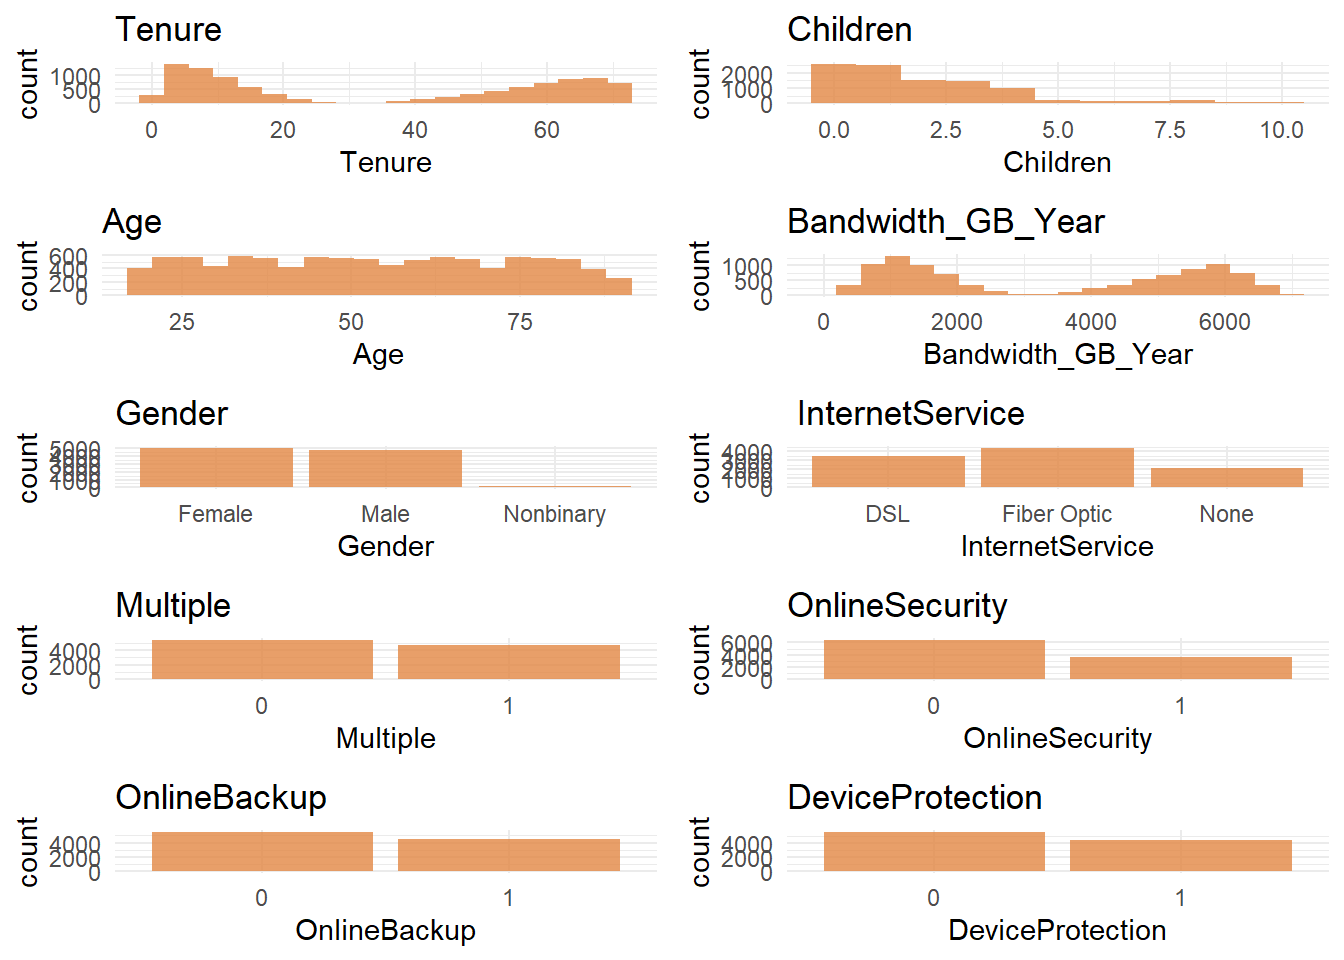
\includegraphics[keepaspectratio]{WriteUpV1_files/figure-latex/unnamed-chunk-4-1.pdf}}

\paragraph{Bivariate Distribution
Plots:}\label{bivariate-distribution-plots}

\pandocbounded{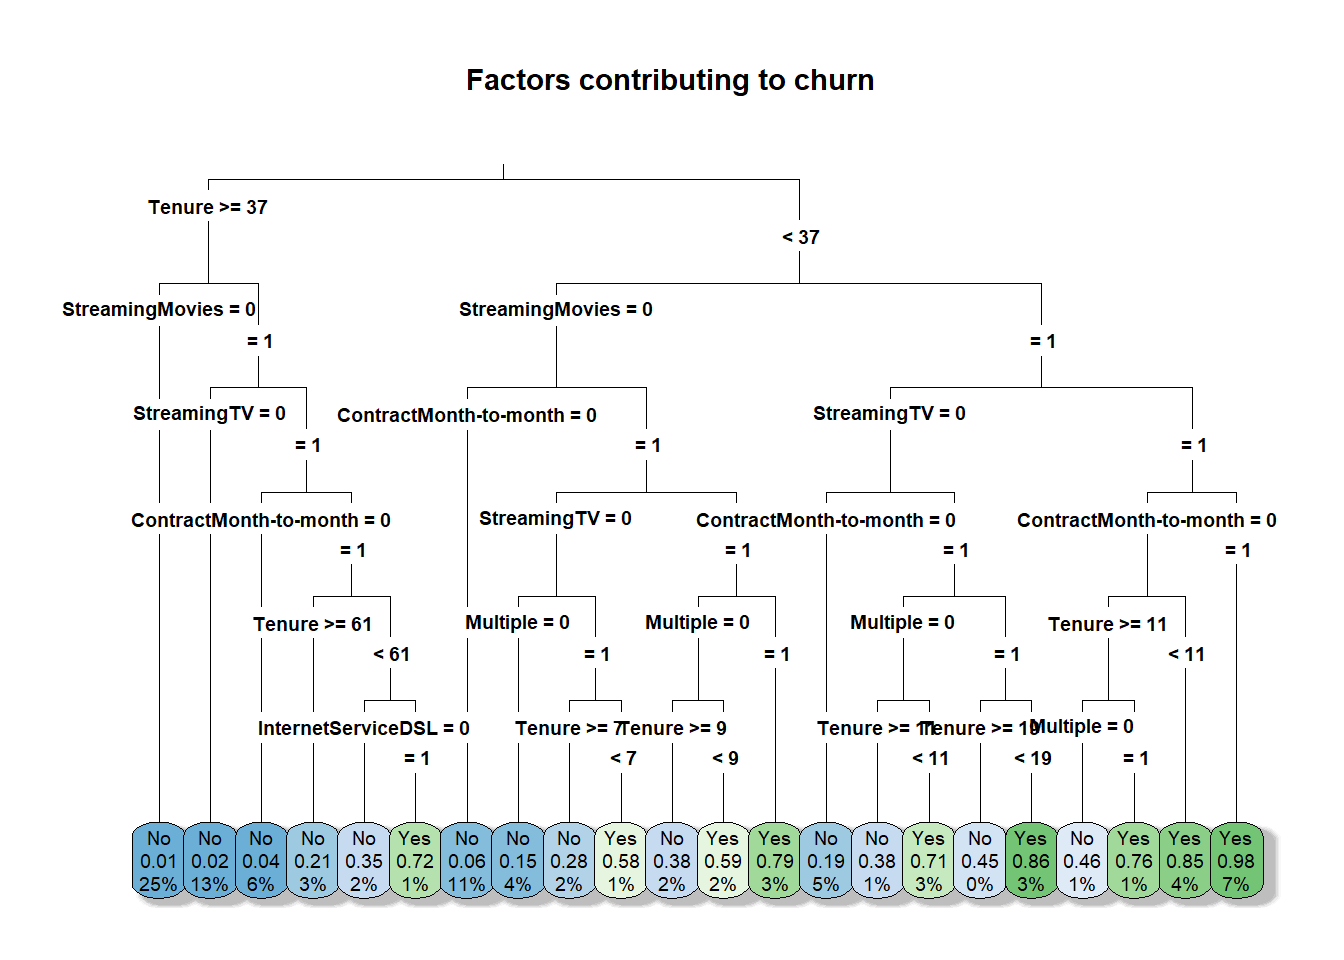
\includegraphics[keepaspectratio]{WriteUpV1_files/figure-latex/unnamed-chunk-5-1.pdf}}

\textbf{C4.} To begin with I will check for na values and duplicates.
For linear regression to work properly I neeed to make sure all the data
is the appropriate type. To do this I will be converting the survey
responses to `factor' while changing the names of the survey columns to
be more intuitive.~ Next I will convert the remaining categorical
columns to factors and the quantitative columns will be converted to
integer or numeric depending on the values.~~

I need to drop irrelevant columns and convert data types to more
appropriate ones to prepare the data. Some categorical variables have
more than 8000 unique entries, which will also be dropped. I will not
create any dummy variables because R automatically creates dummy
variables or indicator variables in the linear model when a categorical
variable is passed into the left of the ``\textasciitilde{}'', so long
as the categorical variable is a factor datatype
\textbf{(Çetinkaya-Rundel et al., 2021)}.\\
\strut \\

\textbf{C5.} The prepared data set will be included in the uploaded
documents. I have named it ``CLEANED\_churn.csv.''\\
Part IV: Model Comparison and Analysis

\section{Part IV: Model Comparison and
Analysis}\label{part-iv-model-comparison-and-analysis}

\textbf{D1.}~ I created an initial model using all the variables
mentioned in C2 by using the ``\textasciitilde{} ., data = churn''
method. Using a ``.'' to the right of the tilda will include all
variables in the data set.~

\begin{Shaded}
\begin{Highlighting}[]
\FunctionTok{summary}\NormalTok{(Initial\_model)}
\end{Highlighting}
\end{Shaded}

\begin{verbatim}
## 
## Call:
## lm(formula = Tenure ~ ., data = training_set)
## 
## Residuals:
##      Min       1Q   Median       3Q      Max 
## -0.15449 -0.10738  0.07453  0.10508  0.16148 
## 
## Coefficients:
##                                        Estimate Std. Error   t value Pr(>|t|)
## (Intercept)                          -3.836e+00  2.854e-02  -134.392  < 2e-16
## Population                           -2.747e-09  8.908e-08    -0.031  0.97540
## AreaSuburban                         -9.197e-03  3.169e-03    -2.903  0.00371
## AreaUrban                            -4.122e-03  3.156e-03    -1.306  0.19157
## Children                             -3.760e-01  6.012e-04  -625.330  < 2e-16
## Age                                   3.997e-02  6.196e-05   645.016  < 2e-16
## Income                                2.536e-08  4.610e-08     0.550  0.58225
## MaritalMarried                       -3.994e-03  4.106e-03    -0.973  0.33074
## MaritalNever Married                 -4.323e-04  4.050e-03    -0.107  0.91499
## MaritalSeparated                      4.931e-04  4.021e-03     0.123  0.90241
## MaritalWidowed                       -1.961e-03  4.008e-03    -0.489  0.62458
## GenderMale                           -7.917e-01  2.620e-03  -302.139  < 2e-16
## GenderNonbinary                       2.659e-01  8.691e-03    30.595  < 2e-16
## Churn1                                1.785e-03  4.128e-03     0.432  0.66541
## Outage_sec_perweek                    1.670e-04  4.330e-04     0.386  0.69969
## Email                                -3.520e-04  4.265e-04    -0.825  0.40919
## Contacts                              2.299e-04  1.296e-03     0.177  0.85921
## Yearly_equip_failure                  4.083e-04  2.035e-03     0.201  0.84097
## Techie1                              -1.266e-03  3.441e-03    -0.368  0.71296
## ContractOne year                      3.730e-03  3.474e-03     1.074  0.28300
## ContractTwo Year                      4.570e-03  3.294e-03     1.387  0.16534
## Port_modem1                          -5.566e-04  2.585e-03    -0.215  0.82952
## Tablet1                               2.625e-03  2.814e-03     0.933  0.35102
## InternetServiceFiber Optic            5.752e+00  4.262e-03  1349.615  < 2e-16
## InternetServiceNone                   4.600e+00  4.061e-03  1132.949  < 2e-16
## Phone1                               -3.347e-04  4.428e-03    -0.076  0.93975
## Multiple1                             2.672e-01  5.462e-03    48.912  < 2e-16
## OnlineSecurity1                      -8.315e-01  2.726e-03  -305.026  < 2e-16
## OnlineBackup1                        -3.566e-01  4.215e-03   -84.606  < 2e-16
## DeviceProtection1                    -5.956e-01  3.189e-03  -186.737  < 2e-16
## TechSupport1                          3.827e-01  3.280e-03   116.681  < 2e-16
## StreamingTV1                         -1.303e+00  6.703e-03  -194.425  < 2e-16
## StreamingMovies1                     -7.270e-01  8.119e-03   -89.536  < 2e-16
## PaperlessBilling1                    -5.597e-03  2.622e-03    -2.135  0.03281
## PaymentMethodCredit Card (automatic)  3.892e-03  3.935e-03     0.989  0.32275
## PaymentMethodElectronic Check         5.075e-03  3.522e-03     1.441  0.14967
## PaymentMethodMailed Check             1.171e-02  3.847e-03     3.045  0.00234
## MonthlyCharge                        -3.513e-02  1.486e-04  -236.363  < 2e-16
## Bandwidth_GB_Year                     1.221e-02  7.199e-07 16953.219  < 2e-16
## Timely_response2                      9.895e-03  9.963e-03     0.993  0.32066
## Timely_response3                      1.445e-02  1.010e-02     1.431  0.15252
## Timely_response4                      1.366e-02  1.050e-02     1.301  0.19321
## Timely_response5                      1.611e-02  1.124e-02     1.433  0.15182
## Timely_response6                      2.188e-02  1.485e-02     1.474  0.14056
## Timely_response7                      4.769e-02  3.151e-02     1.513  0.13025
## Timely_fixes2                        -7.977e-03  1.046e-02    -0.762  0.44591
## Timely_fixes3                        -8.362e-03  1.054e-02    -0.794  0.42751
## Timely_fixes4                        -1.041e-02  1.081e-02    -0.963  0.33565
## Timely_fixes5                        -8.773e-03  1.139e-02    -0.770  0.44126
## Timely_fixes6                        -9.267e-03  1.454e-02    -0.637  0.52405
## Timely_fixes7                        -4.466e-03  3.843e-02    -0.116  0.90750
## Timely_replacements2                  1.336e-03  9.985e-03     0.134  0.89360
## Timely_replacements3                 -3.354e-05  9.893e-03    -0.003  0.99729
## Timely_replacements4                 -8.901e-04  1.009e-02    -0.088  0.92970
## Timely_replacements5                 -1.341e-03  1.067e-02    -0.126  0.90004
## Timely_replacements6                  1.615e-02  1.400e-02     1.154  0.24856
## Timely_replacements7                 -1.270e-02  4.019e-02    -0.316  0.75201
## Timely_replacements8                 -1.265e-01  1.173e-01    -1.078  0.28095
## Reliability2                          5.398e-03  9.471e-03     0.570  0.56871
## Reliability3                          8.658e-03  9.171e-03     0.944  0.34514
## Reliability4                          8.070e-03  9.280e-03     0.870  0.38455
## Reliability5                          1.014e-02  9.807e-03     1.034  0.30129
## Reliability6                          1.247e-02  1.291e-02     0.966  0.33414
## Reliability7                         -5.801e-02  4.926e-02    -1.178  0.23895
## Options2                             -5.206e-03  1.001e-02    -0.520  0.60313
## Options3                             -1.358e-04  9.795e-03    -0.014  0.98894
## Options4                             -2.938e-03  9.917e-03    -0.296  0.76702
## Options5                             -6.652e-03  1.049e-02    -0.634  0.52604
## Options6                             -5.246e-04  1.347e-02    -0.039  0.96895
## Options7                             -1.273e-02  4.212e-02    -0.302  0.76256
## Respectful2                           1.785e-02  1.038e-02     1.720  0.08549
## Respectful3                           1.147e-02  1.024e-02     1.121  0.26250
## Respectful4                           7.977e-03  1.043e-02     0.765  0.44448
## Respectful5                           1.212e-02  1.096e-02     1.106  0.26870
## Respectful6                           1.680e-02  1.396e-02     1.203  0.22891
## Respectful7                           2.612e-02  4.600e-02     0.568  0.57020
## Courteous2                           -4.706e-05  9.430e-03    -0.005  0.99602
## Courteous3                           -4.863e-03  9.125e-03    -0.533  0.59411
## Courteous4                           -6.409e-03  9.235e-03    -0.694  0.48775
## Courteous5                           -2.742e-03  9.775e-03    -0.281  0.77909
## Courteous6                           -4.428e-03  1.283e-02    -0.345  0.73006
## Courteous7                           -3.093e-02  3.743e-02    -0.826  0.40869
## Active_listening2                    -2.888e-02  9.648e-03    -2.993  0.00277
## Active_listening3                    -2.234e-02  9.309e-03    -2.400  0.01643
## Active_listening4                    -2.334e-02  9.385e-03    -2.487  0.01292
## Active_listening5                    -2.514e-02  9.869e-03    -2.548  0.01087
## Active_listening6                    -1.507e-02  1.304e-02    -1.155  0.24795
## Active_listening7                     2.600e-03  3.412e-02     0.076  0.93926
## Active_listening8                    -1.562e-01  1.097e-01    -1.424  0.15455
##                                         
## (Intercept)                          ***
## Population                              
## AreaSuburban                         ** 
## AreaUrban                               
## Children                             ***
## Age                                  ***
## Income                                  
## MaritalMarried                          
## MaritalNever Married                    
## MaritalSeparated                        
## MaritalWidowed                          
## GenderMale                           ***
## GenderNonbinary                      ***
## Churn1                                  
## Outage_sec_perweek                      
## Email                                   
## Contacts                                
## Yearly_equip_failure                    
## Techie1                                 
## ContractOne year                        
## ContractTwo Year                        
## Port_modem1                             
## Tablet1                                 
## InternetServiceFiber Optic           ***
## InternetServiceNone                  ***
## Phone1                                  
## Multiple1                            ***
## OnlineSecurity1                      ***
## OnlineBackup1                        ***
## DeviceProtection1                    ***
## TechSupport1                         ***
## StreamingTV1                         ***
## StreamingMovies1                     ***
## PaperlessBilling1                    *  
## PaymentMethodCredit Card (automatic)    
## PaymentMethodElectronic Check           
## PaymentMethodMailed Check            ** 
## MonthlyCharge                        ***
## Bandwidth_GB_Year                    ***
## Timely_response2                        
## Timely_response3                        
## Timely_response4                        
## Timely_response5                        
## Timely_response6                        
## Timely_response7                        
## Timely_fixes2                           
## Timely_fixes3                           
## Timely_fixes4                           
## Timely_fixes5                           
## Timely_fixes6                           
## Timely_fixes7                           
## Timely_replacements2                    
## Timely_replacements3                    
## Timely_replacements4                    
## Timely_replacements5                    
## Timely_replacements6                    
## Timely_replacements7                    
## Timely_replacements8                    
## Reliability2                            
## Reliability3                            
## Reliability4                            
## Reliability5                            
## Reliability6                            
## Reliability7                            
## Options2                                
## Options3                                
## Options4                                
## Options5                                
## Options6                                
## Options7                                
## Respectful2                          .  
## Respectful3                             
## Respectful4                             
## Respectful5                             
## Respectful6                             
## Respectful7                             
## Courteous2                              
## Courteous3                              
## Courteous4                              
## Courteous5                              
## Courteous6                              
## Courteous7                              
## Active_listening2                    ** 
## Active_listening3                    *  
## Active_listening4                    *  
## Active_listening5                    *  
## Active_listening6                       
## Active_listening7                       
## Active_listening8                       
## ---
## Signif. codes:  0 '***' 0.001 '**' 0.01 '*' 0.05 '.' 0.1 ' ' 1
## 
## Residual standard error: 0.1075 on 6911 degrees of freedom
## Multiple R-squared:      1,  Adjusted R-squared:      1 
## F-statistic: 4.799e+06 on 88 and 6911 DF,  p-value: < 2.2e-16
\end{verbatim}

\textbf{D2.} After running the initial linear model from the training
set (``Initial\_model'')~it became apparent that there were several
values that were not statistically significant as noted by the lack of
the
\pandocbounded{\includegraphics[keepaspectratio]{https://lh7-rt.googleusercontent.com/docsz/AD_4nXe5VNjtMQSILD2pI0shhZtLtH-9os-62mspk6YayIYbUurztTNQUyfDP2EmJ2m7opZnO7gK8RrpsRGNV0X26vtSuR9NOBJ-d609ViFOYEhBXcD74x4CWnmGkHASh3iQqP5szgZmww?key=SXQIj9I0Eg3DnjP4XZcTs35-}}marking
that indicates that the values are statistically significant. I've
chosen to use backward stepwise selection \textbf{(Larose \& Larose,
2019)}, and created a model named ``stepwise\_model'', because I have a
large amount of variables and backward elimination will remove each
insignificant variable until only those values that have a meaningful
contribution will remain.~

The following table shows that this dimension reduction technique
successfully decreased the amount of variables that would be included in
the final model. However, \emph{``PaymentMethodElectronic Check''},
\emph{``PaymentMethodCredit Card (automatic)''}, and
\emph{``AreaUrban''} all have p-values that are greater than 0.05
indicating that these are not contributing significantly to the model.
So, I looked at the Variance Inflation Factor (VIF) values of the
stepwise model to check multicollinearity.~

\begin{Shaded}
\begin{Highlighting}[]
\FunctionTok{summary}\NormalTok{(Initial\_model)}
\end{Highlighting}
\end{Shaded}

\begin{verbatim}
## 
## Call:
## lm(formula = Tenure ~ Area + Children + Age + Gender + InternetService + 
##     Multiple + OnlineSecurity + OnlineBackup + DeviceProtection + 
##     TechSupport + StreamingTV + StreamingMovies + PaperlessBilling + 
##     PaymentMethod + MonthlyCharge + Bandwidth_GB_Year, data = training_set)
## 
## Residuals:
##      Min       1Q   Median       3Q      Max 
## -0.13667 -0.10827  0.08645  0.10502  0.13507 
## 
## Coefficients:
##                                        Estimate Std. Error   t value Pr(>|t|)
## (Intercept)                          -3.841e+00  1.390e-02  -276.328  < 2e-16
## AreaSuburban                         -9.128e-03  3.150e-03    -2.898  0.00377
## AreaUrban                            -4.160e-03  3.137e-03    -1.326  0.18491
## Children                             -3.759e-01  5.974e-04  -629.244  < 2e-16
## Age                                   3.996e-02  6.160e-05   648.726  < 2e-16
## GenderMale                           -7.921e-01  2.600e-03  -304.618  < 2e-16
## GenderNonbinary                       2.646e-01  8.636e-03    30.635  < 2e-16
## InternetServiceFiber Optic            5.752e+00  4.124e-03  1394.903  < 2e-16
## InternetServiceNone                   4.600e+00  4.021e-03  1144.221  < 2e-16
## Multiple1                             2.679e-01  5.417e-03    49.451  < 2e-16
## OnlineSecurity1                      -8.314e-01  2.709e-03  -306.867  < 2e-16
## OnlineBackup1                        -3.564e-01  4.178e-03   -85.302  < 2e-16
## DeviceProtection1                    -5.953e-01  3.170e-03  -187.808  < 2e-16
## TechSupport1                          3.830e-01  3.247e-03   117.938  < 2e-16
## StreamingTV1                         -1.302e+00  6.659e-03  -195.546  < 2e-16
## StreamingMovies1                     -7.261e-01  8.067e-03   -90.003  < 2e-16
## PaperlessBilling1                    -5.113e-03  2.604e-03    -1.963  0.04964
## PaymentMethodCredit Card (automatic)  3.828e-03  3.910e-03     0.979  0.32763
## PaymentMethodElectronic Check         5.123e-03  3.496e-03     1.466  0.14282
## PaymentMethodMailed Check             1.138e-02  3.820e-03     2.979  0.00290
## MonthlyCharge                        -3.514e-02  1.460e-04  -240.680  < 2e-16
## Bandwidth_GB_Year                     1.220e-02  5.940e-07 20546.755  < 2e-16
##                                         
## (Intercept)                          ***
## AreaSuburban                         ** 
## AreaUrban                               
## Children                             ***
## Age                                  ***
## GenderMale                           ***
## GenderNonbinary                      ***
## InternetServiceFiber Optic           ***
## InternetServiceNone                  ***
## Multiple1                            ***
## OnlineSecurity1                      ***
## OnlineBackup1                        ***
## DeviceProtection1                    ***
## TechSupport1                         ***
## StreamingTV1                         ***
## StreamingMovies1                     ***
## PaperlessBilling1                    *  
## PaymentMethodCredit Card (automatic)    
## PaymentMethodElectronic Check           
## PaymentMethodMailed Check            ** 
## MonthlyCharge                        ***
## Bandwidth_GB_Year                    ***
## ---
## Signif. codes:  0 '***' 0.001 '**' 0.01 '*' 0.05 '.' 0.1 ' ' 1
## 
## Residual standard error: 0.1073 on 6978 degrees of freedom
## Multiple R-squared:      1,  Adjusted R-squared:      1 
## F-statistic: 2.017e+07 on 21 and 6978 DF,  p-value: < 2.2e-16
\end{verbatim}

According to Zach Bobbitt from statology, ``A value greater than 5
indicates potentially severe correlation between a given predictor
variable and other predictor variables in the model. In this case, the
coefficient estimates and p-values in the regression output are likely
unreliable. \textbf{(Z. Bobbitt, 2019)}.''~ So, I looked for all VIF
values above 5.

\begin{Shaded}
\begin{Highlighting}[]
\NormalTok{vif\_values }\OtherTok{\textless{}{-}} \FunctionTok{vif}\NormalTok{(Initial\_model)}
\NormalTok{vif\_values }\CommentTok{\#Looking for VIF values above 5. }
\end{Highlighting}
\end{Shaded}

\begin{verbatim}
##                        GVIF Df GVIF^(1/(2*Df))
## Area               1.004114  2        1.001027
## Children           1.002341  1        1.001170
## Age                1.003046  1        1.001522
## Gender             1.006402  2        1.001597
## InternetService    3.285748  2        1.346352
## Multiple           4.427459  1        2.104153
## OnlineSecurity     1.025144  1        1.012494
## OnlineBackup       2.623569  1        1.619743
## DeviceProtection   1.503409  1        1.226136
## TechSupport        1.492439  1        1.221654
## StreamingTV        6.737752  1        2.595718
## StreamingMovies    9.882268  1        3.143607
## PaperlessBilling   1.002978  1        1.001488
## PaymentMethod      1.005897  3        1.000980
## MonthlyCharge     23.873153  1        4.886016
## Bandwidth_GB_Year  1.022208  1        1.011043
\end{verbatim}

As you can see, StreamingTV, StreamingMovies, and MonthlyCharge all had
VIF values above 5.~ Because MonthlyCharge was so much higher than the
rest, I decided to remove it first and see if that made the others
acceptable.

\begin{Shaded}
\begin{Highlighting}[]
\NormalTok{vif\_values }\OtherTok{\textless{}{-}} \FunctionTok{vif}\NormalTok{(Initial\_model)}
\NormalTok{vif\_values }\CommentTok{\#Looking for VIF values above 5. }
\end{Highlighting}
\end{Shaded}

\begin{verbatim}
##                        GVIF Df GVIF^(1/(2*Df))
## Area               1.004114  2        1.001027
## Children           1.002341  1        1.001170
## Age                1.003046  1        1.001522
## Gender             1.006402  2        1.001597
## InternetService    3.285748  2        1.346352
## Multiple           4.427459  1        2.104153
## OnlineSecurity     1.025144  1        1.012494
## OnlineBackup       2.623569  1        1.619743
## DeviceProtection   1.503409  1        1.226136
## TechSupport        1.492439  1        1.221654
## StreamingTV        6.737752  1        2.595718
## StreamingMovies    9.882268  1        3.143607
## PaperlessBilling   1.002978  1        1.001488
## PaymentMethod      1.005897  3        1.000980
## MonthlyCharge     23.873153  1        4.886016
## Bandwidth_GB_Year  1.022208  1        1.011043
\end{verbatim}

\begin{Shaded}
\begin{Highlighting}[]
\CommentTok{\# Removed MonthlyCharge since it was such a high VIF and then i will check VIF again to see if the others are ok}
\NormalTok{reduced\_model }\OtherTok{\textless{}{-}} \FunctionTok{lm}\NormalTok{(}\AttributeTok{formula =}\NormalTok{ Tenure }\SpecialCharTok{\textasciitilde{}}\NormalTok{ Area }\SpecialCharTok{+}\NormalTok{ Children }\SpecialCharTok{+}\NormalTok{ Age }\SpecialCharTok{+}\NormalTok{ Gender }\SpecialCharTok{+}\NormalTok{ InternetService }\SpecialCharTok{+}\NormalTok{ Multiple }\SpecialCharTok{+}\NormalTok{ OnlineSecurity }\SpecialCharTok{+}\NormalTok{ OnlineBackup }\SpecialCharTok{+}\NormalTok{ DeviceProtection }\SpecialCharTok{+}\NormalTok{ TechSupport }\SpecialCharTok{+}\NormalTok{ StreamingTV }\SpecialCharTok{+}\NormalTok{ StreamingMovies }\SpecialCharTok{+}\NormalTok{ PaperlessBilling }\SpecialCharTok{+}\NormalTok{ PaymentMethod }\SpecialCharTok{+}\NormalTok{ Bandwidth\_GB\_Year, }\AttributeTok{data =}\NormalTok{ churn)}

\FunctionTok{summary}\NormalTok{(reduced\_model)}
\end{Highlighting}
\end{Shaded}

\begin{verbatim}
## 
## Call:
## lm(formula = Tenure ~ Area + Children + Age + Gender + InternetService + 
##     Multiple + OnlineSecurity + OnlineBackup + DeviceProtection + 
##     TechSupport + StreamingTV + StreamingMovies + PaperlessBilling + 
##     PaymentMethod + Bandwidth_GB_Year, data = churn)
## 
## Residuals:
##     Min      1Q  Median      3Q     Max 
## -0.4652 -0.2355  0.1757  0.3843  0.4479 
## 
## Coefficients:
##                                        Estimate Std. Error  t value Pr(>|t|)
## (Intercept)                          -6.783e+00  1.685e-02 -402.603   <2e-16
## AreaSuburban                         -9.006e-03  8.028e-03   -1.122    0.262
## AreaUrban                            -3.601e-03  8.042e-03   -0.448    0.654
## Children                             -3.759e-01  1.528e-03 -245.924   <2e-16
## Age                                   3.987e-02  1.586e-04  251.398   <2e-16
## GenderMale                           -7.834e-01  6.642e-03 -117.958   <2e-16
## GenderNonbinary                       2.913e-01  2.208e-02   13.194   <2e-16
## InternetServiceFiber Optic            5.055e+00  7.483e-03  675.584   <2e-16
## InternetServiceNone                   5.054e+00  9.063e-03  557.615   <2e-16
## Multiple1                            -8.790e-01  6.580e-03 -133.576   <2e-16
## OnlineSecurity1                      -9.253e-01  6.846e-03 -135.168   <2e-16
## OnlineBackup1                        -1.150e+00  6.599e-03 -174.196   <2e-16
## DeviceProtection1                    -1.038e+00  6.612e-03 -156.950   <2e-16
## TechSupport1                         -5.701e-02  6.777e-03   -8.411   <2e-16
## StreamingTV1                         -2.783e+00  6.569e-03 -423.675   <2e-16
## StreamingMovies1                     -2.564e+00  6.568e-03 -390.369   <2e-16
## PaperlessBilling1                    -9.508e-03  6.664e-03   -1.427    0.154
## PaymentMethodCredit Card (automatic)  1.069e-02  9.997e-03    1.070    0.285
## PaymentMethodElectronic Check         5.365e-03  8.940e-03    0.600    0.548
## PaymentMethodMailed Check             7.493e-03  9.761e-03    0.768    0.443
## Bandwidth_GB_Year                     1.220e-02  1.515e-06 8055.715   <2e-16
##                                         
## (Intercept)                          ***
## AreaSuburban                            
## AreaUrban                               
## Children                             ***
## Age                                  ***
## GenderMale                           ***
## GenderNonbinary                      ***
## InternetServiceFiber Optic           ***
## InternetServiceNone                  ***
## Multiple1                            ***
## OnlineSecurity1                      ***
## OnlineBackup1                        ***
## DeviceProtection1                    ***
## TechSupport1                         ***
## StreamingTV1                         ***
## StreamingMovies1                     ***
## PaperlessBilling1                       
## PaymentMethodCredit Card (automatic)    
## PaymentMethodElectronic Check           
## PaymentMethodMailed Check               
## Bandwidth_GB_Year                    ***
## ---
## Signif. codes:  0 '***' 0.001 '**' 0.01 '*' 0.05 '.' 0.1 ' ' 1
## 
## Residual standard error: 0.3278 on 9979 degrees of freedom
## Multiple R-squared:  0.9998, Adjusted R-squared:  0.9998 
## F-statistic: 3.254e+06 on 20 and 9979 DF,  p-value: < 2.2e-16
\end{verbatim}

I found that after removing MonthlyCharge with a VIF of 23.87, the model
returned ``AreaSuburban'', ``AreaUrban'', ``PaperlessBilling1,''
``PaymentMethodCredit Card (automatic),'' ``PaymentMethodElectronic
Check,'' ``PaymentMethodMailed Check'' to all have values that were not
statistically significant. The following table is the result of the
second stepwise elimination. I checked the VIF values for the updated
model and found all values around 1.

\begin{Shaded}
\begin{Highlighting}[]
\FunctionTok{summary}\NormalTok{(reduced\_model)}
\end{Highlighting}
\end{Shaded}

\begin{verbatim}
## 
## Call:
## lm(formula = Tenure ~ Children + Age + Gender + InternetService + 
##     Multiple + OnlineSecurity + OnlineBackup + DeviceProtection + 
##     TechSupport + StreamingTV + StreamingMovies + Bandwidth_GB_Year, 
##     data = churn)
## 
## Residuals:
##     Min      1Q  Median      3Q     Max 
## -0.4536 -0.2314  0.1829  0.3839  0.4400 
## 
## Coefficients:
##                              Estimate Std. Error  t value Pr(>|t|)    
## (Intercept)                -6.787e+00  1.443e-02 -470.301   <2e-16 ***
## Children                   -3.759e-01  1.528e-03 -245.959   <2e-16 ***
## Age                         3.987e-02  1.585e-04  251.483   <2e-16 ***
## GenderMale                 -7.833e-01  6.638e-03 -117.996   <2e-16 ***
## GenderNonbinary             2.913e-01  2.207e-02   13.197   <2e-16 ***
## InternetServiceFiber Optic  5.055e+00  7.479e-03  675.955   <2e-16 ***
## InternetServiceNone         5.054e+00  9.061e-03  557.742   <2e-16 ***
## Multiple1                  -8.790e-01  6.579e-03 -133.614   <2e-16 ***
## OnlineSecurity1            -9.253e-01  6.844e-03 -135.205   <2e-16 ***
## OnlineBackup1              -1.150e+00  6.597e-03 -174.256   <2e-16 ***
## DeviceProtection1          -1.038e+00  6.610e-03 -157.026   <2e-16 ***
## TechSupport1               -5.700e-02  6.775e-03   -8.412   <2e-16 ***
## StreamingTV1               -2.783e+00  6.567e-03 -423.764   <2e-16 ***
## StreamingMovies1           -2.564e+00  6.567e-03 -390.448   <2e-16 ***
## Bandwidth_GB_Year           1.220e-02  1.514e-06 8058.672   <2e-16 ***
## ---
## Signif. codes:  0 '***' 0.001 '**' 0.01 '*' 0.05 '.' 0.1 ' ' 1
## 
## Residual standard error: 0.3277 on 9985 degrees of freedom
## Multiple R-squared:  0.9998, Adjusted R-squared:  0.9998 
## F-statistic: 4.649e+06 on 14 and 9985 DF,  p-value: < 2.2e-16
\end{verbatim}

\textbf{D3.} The updated model (reduced\_model), includes Tenure
(dependant variable), Children, Age, GenderMale, GenderNonbinary,
InternetServiceFiber Optic, InternetServiceNone, Multiple1,
OnlineSecurity1, OnlineBackup1, DeviceProtection1, TechSupport1,
StreamingTV1, StreamingMovies1, and Bandwidth\_GB\_Year.~

The reduced\_model shows an adjusted R-squared value of 0.9998, meaning
that the model accounts for 99.98\% of variance in Tenure. The models
f-statistic is 4.649e+06 and the p-value is 2.2e-16 which indicates that
the model works and is highly significant. The Residuals range from
-0.4536 to 0.4400 with a median of 0.1829. In this new model, all of the
preidictor variabels are statistically significant.

\textbf{E1}. To compare the initial model and the reduced model, I used
a kruskal-wallis test as opposed to an ANOVA becuase ANOVA assumes a
normal distribution. Because the residuals are not normally distributed
I used a non-parametric alternative to the ANOVA, known as the
Kruskal-wallis test.\\

\begin{Shaded}
\begin{Highlighting}[]
\CommentTok{\# comparing the residuals of each model.}
\FunctionTok{kruskal.test}\NormalTok{(Residuals }\SpecialCharTok{\textasciitilde{}}\NormalTok{ Model, }\AttributeTok{data =}\NormalTok{ residuals\_df)}
\end{Highlighting}
\end{Shaded}

\begin{verbatim}
## 
##  Kruskal-Wallis rank sum test
## 
## data:  Residuals by Model
## Kruskal-Wallis chi-squared = 1.2851, df = 1, p-value = 0.2569
\end{verbatim}

The Kruskal-Wallis test compares the distributions of residuals between
two models and tests whether their medians are the same. The test
statistic (chi-squared = 1.2851) with 1 degree of freedom returned a
p-value of 0.2569, indicating no significant difference between the
residual distributions of the models. This suggests that the residuals
from both models are similar in distribution. Because the p-value is
greater than 0.05, I fail to reject the null hypothesis that there is no
difference between the distribution of the residuals in each model.

\textbf{E2.} I will include the full code file in my assessment uploads.

The reduced model has a residual standard error of 0.3277 and a adjusted
r-squared value of 0.9998. This suggests that the model has very good
fit. In terms of predictive power, this residual standard error
indicates that the reduced model provides very precise predictions.

\pandocbounded{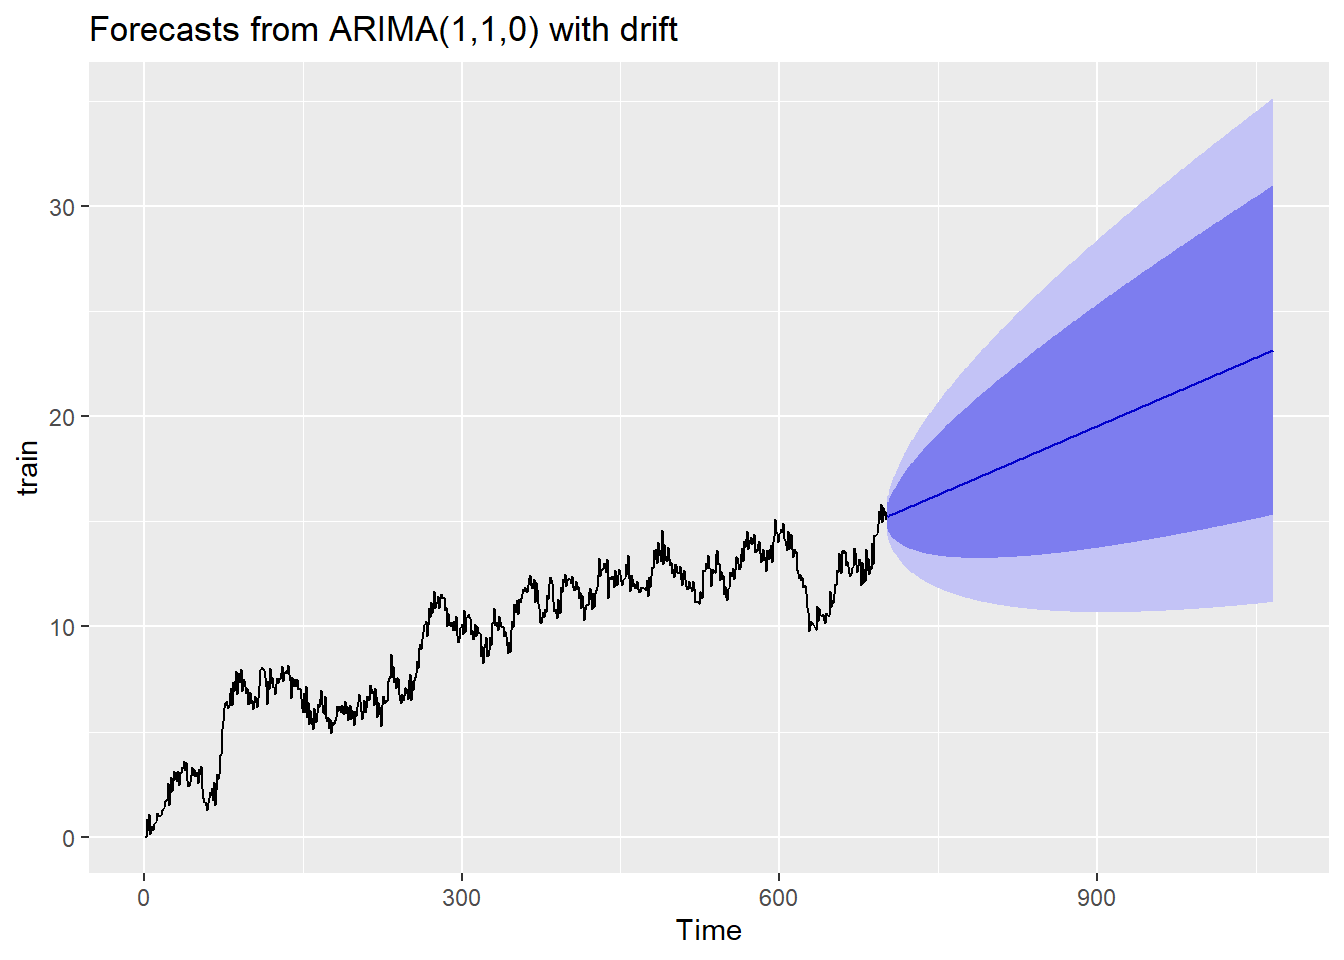
\includegraphics[keepaspectratio]{WriteUpV1_files/figure-latex/unnamed-chunk-16-1.pdf}}

The \textbf{residuals vs leverage} (bottom right) plot shows that there
are no high leverage point or outliers based on `cooks distance.'

The \textbf{Q-Q residuals} plot (top right) show that the residuals do
not stick to the diagonal line expecially on the tails indicating that
the residuals are not normally distributed.

The r\textbf{esiduals vs fitted} (top left)plot show that the horizontal
red line is reasonably flat but the residuals show horizontal lines
rather than randomness suggesting heteroscadasticity rather than the
assumption of homoscedasticity.

The \textbf{scale-location} (bottom left) plot checks for
homoscedasticity. Once again the residuals show horizontal lines.
Ideally these values should be evenly spread across the plot.

\section{Part V: Data Summary and
Implications}\label{part-v-data-summary-and-implications}

\textbf{F1.} In this model, the Y-intercept is not particularly
meaningful because many of the variables do not have practical
interpretations when equal to zero. For example, an age of zero would
imply the presence of customers who are newborns, which is unrealistic.
Additionally, some variables are binary, where a value of zero
represents ``No.'' In other words, when all predictors are zero, the
expected value of tenure would be -6.787 months, which dosen't make
sense. So the Y-intercept in this context is not meaningful.

The model has a statistically significant p-value meaning that I can
reject the null hypothesis that the predictors have no effect on tenure.
In this particular model, InternetServiceFiber Optic and
InternetServiceNone have the highest positive coefficients (5.055 and
5.054) meaning that the customers with fiber optic service or no
internet service are associated with higher tenure. in contrast, it
appeas that the two variables with the most negative coeefficients,
StreamingTV1 and StreamingMovies1 (-2.783 and -2.564) are both
associated with customers who have lower tenure.

\textbf{F2.} This model can identify discrepancies between predicted and
actual customer tenure, which is critical for mitigating churn. For
example, if the model predicts a customer's tenure to be 18 months, but
their actual tenure reaches 24 months, it could signal imminent churn.
In such cases, the company should take proactive measures such as
offering service upgrades, discounts, or addressing potential
dissatisfaction to retain the customer. Similarly, if a customer is
predicted to stay for 24 months, but by 18 months their usage declines
or their customer service calls increase, this could indicate early
signs of churn that require prompt intervention.

Additionally, the model can predict expected tenure for new customers
based on demographics and service usage patterns. Insights from key
predictors, such as the positive impact of ``\emph{InternetServiceFiber
Optic''} and the negative impact of''\emph{StreamingTV},'' enable the
company to tailor offerings. For example, promoting fiber-optic services
or improving streaming-related issues could enhance retention among
customers with a higher risk of shorter tenure.

\section{Part VI: Demonstration}\label{part-vi-demonstration}

\textbf{G.} A link to the panopto demonstration video will be included
in the uploaded documents.

\textbf{H:} Web Sources:

\begin{enumerate}
\def\labelenumi{\arabic{enumi}.}
\item
  \textbf{Bobbitt, Z. (2019, March 10).} Multicollinearity in
  regression. Statology. Retrieved November 17, 2024, from
  \url{https://www.statology.org/multicollinearity-regression/}
\item
  \textbf{Bobbitt, Z. (2020, January 8).} The four assumptions of linear
  regression. Statology. Retrieved November 17, 2024, from
  \url{https://www.statology.org/linear-regression-assumptions/}
\end{enumerate}

\begin{enumerate}
\def\labelenumi{\arabic{enumi}.}
\setcounter{enumi}{3}
\tightlist
\item
  \textbf{Çetinkaya-Rundel, M., Hardin, J., \& Horton, N. J. (2021).}
  Dummy variables and interactions. Modern Statistics with R. Retrieved
  December 4, 2024, from
  \url{https://www.modernstatisticswithr.com/regression.html\#dummy}
\end{enumerate}

\begin{enumerate}
\def\labelenumi{\arabic{enumi}.}
\setcounter{enumi}{4}
\tightlist
\item
  \textbf{Gallo, A. (2014, October 29).} The value of keeping the right
  customers. Harvard Business Review. Retrieved November 17, 2024, from
  \url{https://hbr.org/2014/10/the-value-of-keeping-the-right-customers}
\end{enumerate}

\begin{enumerate}
\def\labelenumi{\arabic{enumi}.}
\setcounter{enumi}{5}
\tightlist
\item
  \textbf{Ihaka, R. (n.d.).} The R Project: A brief history and thoughts
  about the future (p.~12). The University of Auckland. Retrieved
  November 17, 2024, from
  \url{https://www.stat.auckland.ac.nz/~ihaka/downloads/Otago.pdf}
\end{enumerate}

\begin{enumerate}
\def\labelenumi{\arabic{enumi}.}
\setcounter{enumi}{6}
\tightlist
\item
  \textbf{Larose, C. D., \& Larose, D. T. (2019).} Data science using
  Python and R. Wiley. Retrieved from
  \url{https://eds.p.ebscohost.com/eds/ebookviewer/ebook/bmxlYmtfXzIwOTEzNzFfX0FO0?sid=04ef9475-3bed-4dbe-8317-a1c5eb6da3cb@redis&vid=0&format=EB&lpid=lp_151&rid=0}
\end{enumerate}

\begin{enumerate}
\def\labelenumi{\arabic{enumi}.}
\setcounter{enumi}{7}
\tightlist
\item
  \textbf{Martin, G.} {[}R Programming 101{]}. (n.d.). Multiple
  regression - Making sure that your assumptions are met {[}Video{]}.
  YouTube. \url{https://www.youtube.com/watch?v=1lwvNLDSu0s&t=1092s}
\end{enumerate}

\end{document}
